\section{1.e: Instruction Set architecture Arithmetic}
\begin{parag}{Notation}
    \begin{itemize}
        \item Number (represented on a specific no. of digits/bits)
			\begin{align*} A =  A^{\left(n\right)}  =  A^{\left(m\right)}\end{align*}
		\item  Number (in binary or decimal)
			\begin{align*} A = A_{10} =  A_2 = A_{2c} \end{align*}
			\item Individual digits (bits)
				\begin{align*} a_{n-1}, a_{n-2}, \ldots, a_2, a_1, a_0 \end{align*}
				\item Digit string (representation)
					\begin{align*} <a_{n-1}a_{n-2}\cdots a_2 a_1 a_0> \end{align*}
    \end{itemize}
\end{parag}
\begin{parag}{Numbers}
    we usually care for three types of numbers:
	\begin{itemize}
	    \item \important{Integers} (signed and unsigned)
		\item Fixed point
			\begin{align*} 0.12, 3.14, 1013141212512.5124213 \end{align*}
			\begin{itemize}
			    \item Essentially integers with \important{implicit $10^{k}$ or $2^k$ scaling}
			    \item Extremly important in practice (most signal processing is fixed point)
			\end{itemize}
		\item \important{Floating point}	
			\begin{align*} 3.14E3, -2.4E-1 \end{align*}
	\end{itemize}
	\begin{framedremark}
	As we have seen in it fds, we feel like fixed point are just some useless number representation but this is \important{false}. As said before, in signal processing we use a lot of number that needs to be \textit{pointed} (not integers), but it also need to be \important{fast} as for us to be able to watch a live twitch or a youtube video... We need to do a lot of computation the fastest way possible. Floating point are pretty bad at this, addition using floating is much more slower than integers addition, we know that fixed point are just integers disguised as rational number. That's the reason why we use fixed point representation.
	\end{framedremark}
\end{parag}
\begin{parag}{Unsigned Integers}
    \begin{align*} A = \sum_{i = 0}^{n - 1} a_iR^i \end{align*}
\end{parag}
\begin{framedremark}
For the next part of this course I am gonna skips this because it is a big review of what we have already seen in fds, I am just going to write what I find intresting \textbf{for me} which is not necessarly the most important thing.
\end{framedremark}
\begin{parag}{Addition is unchanged from unsigned}
    As we can see (remember of the table) addition for signed number (in two's complement) and unsigned number is the same, this allows us to have \important{only} two instructions (\texttt{add} and \texttt{sub}) without any \texttt{addu} like instruction.\\
	This is one of the reason why we use 2's complement as the universal representation of signed integers today.
\end{parag}


\begin{parag}{Overflow in hardware}
    In hardware, \important{carry out} is the only missing bit from the \important{complete} result\\
	We can think of overflows as a \important{tuncation} problem:
	\begin{center}
	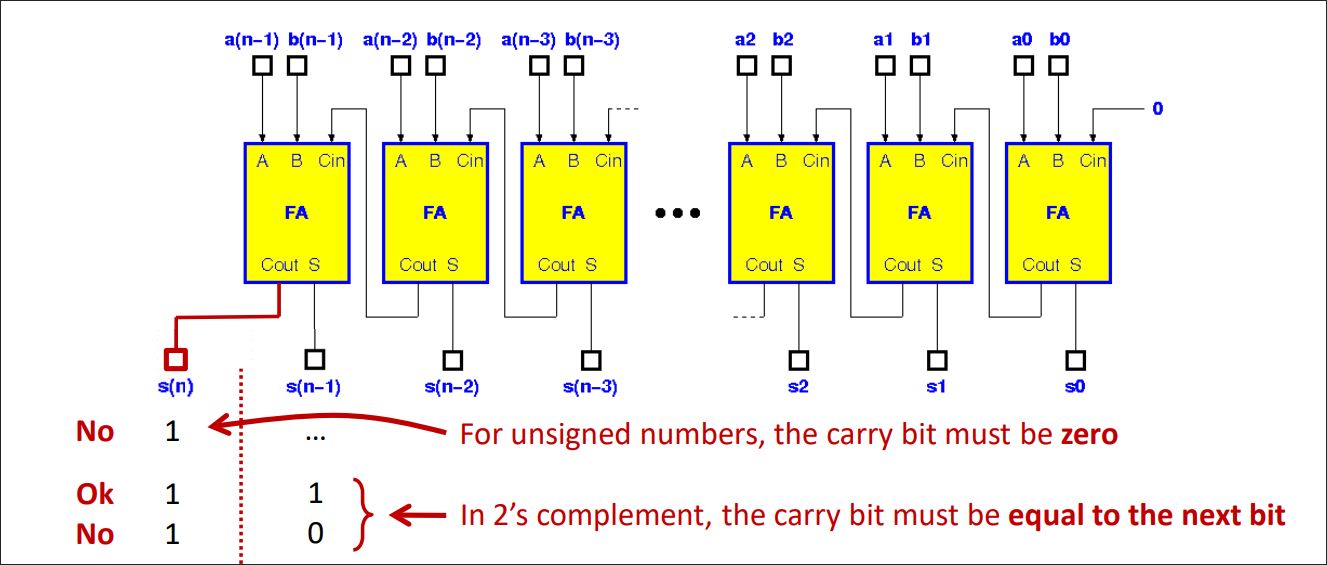
\includegraphics[scale=0.3]{screenshots/2025-10-21_2.png}
	\end{center}
\end{parag}
\begin{parag}{Overflow in software}
    Some architecture (e.g., \important{x86}) gives us the \important{carry bit} in a special register (a \important{flag})
	\begin{center}
	    \textrightarrow overflow detection is the same as in hardware
	\end{center}
	Other modern architecture gives us \important{only the result} of the addition (e.g., \important{RISC-V}). The detection is usually based on the following observations:
	\begin{itemize}
	    \item If addition of \important{opposite sign number} $\implies$ magnitude can only reduce $\to$\important{no overflow possible}
	    \item If addition of \important{same sign number}$\implies$ overflow is possible but the sign of the result will appear wrong.
	\end{itemize}
	
	
	\end{parag}
\begin{parag}{$A + \overline{A} = -1$}
	As we have seen here
	\begin{align*} -A = \overline{A} + 1\end{align*}
	To prove it:
	\begin{align*} &\left(-a_{n-1} 2^{n-1} + \sum_{i =  0}\
		^{n-2}a_i2^i\right) + \left(-\overline{a_{n-1}}2^{n-1} + \sum_{i = 0}^{n-2}\overline{a_i}2^i\right) \\ &= - \left(a_{n-1} + \overline{a_{n-1}}\right) \cdot 2^{n-i} + \sum_{i = 0}^{n-2}\left(a_i + \overline{a_i}\right) \cdot 2^i =  -2^{n-1} + \sum_{i = 0}^{n-2}  2^i\\ &=  -1
\end{align*}
    
\end{parag}
\begin{parag}{Two's complement Add/Subtract Units}
    With this proprety it becomes very easy to compute subtraction as it is just the use of the addition part but with the inverse + 1. This can be done by having a $c_{in}$ at the beggining of the adder and to have a multiplexer to choose between the $b_i$ or $\neg b_i$
	\begin{center}
	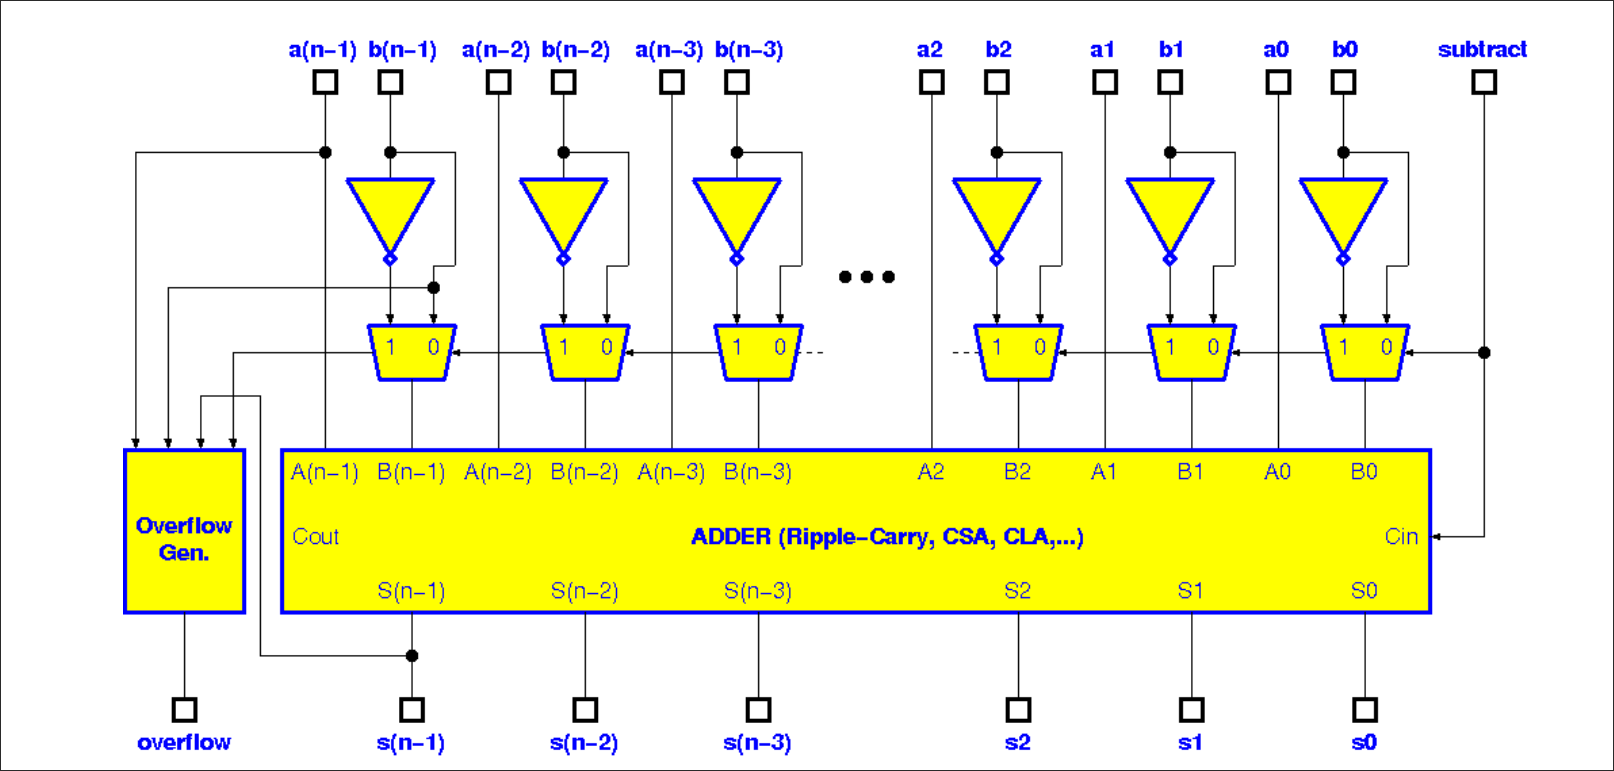
\includegraphics[scale=0.2]{screenshots/2025-10-21_3.png}
	\end{center}
	as we can see this allows us to put the substraction and addition into the same module.
\end{parag}







